\subsection{Conjugate axes and inner-product spaces}\label{sec:conjugate}

For any non-singular $\mat{A}$ in \eqref{eq:ellAS} that generates an ellipsoid,  %% added non-singular / GM
the columns of
$\mat{A}=\left[
   \vec{a}_{1}, \vec{a}_{2}, \cdots, \vec{a}_{p}  \\
\right]
$
form a set of ``conjugate axes'' of the ellipse. (Two diameters are conjugate \emph{iff}
the tangent line at the endpoint of one diameter is parallel to the other diameter.)
Each vector
$\vec{a}_{i}$
lies on the ellipse, and the tangent space at that point is parallel to the span of all the other column vectors of
$\vec{A}$.
\begin{figure}[htb]
 \begin{minipage}[b]{.49\linewidth}
  \centering
  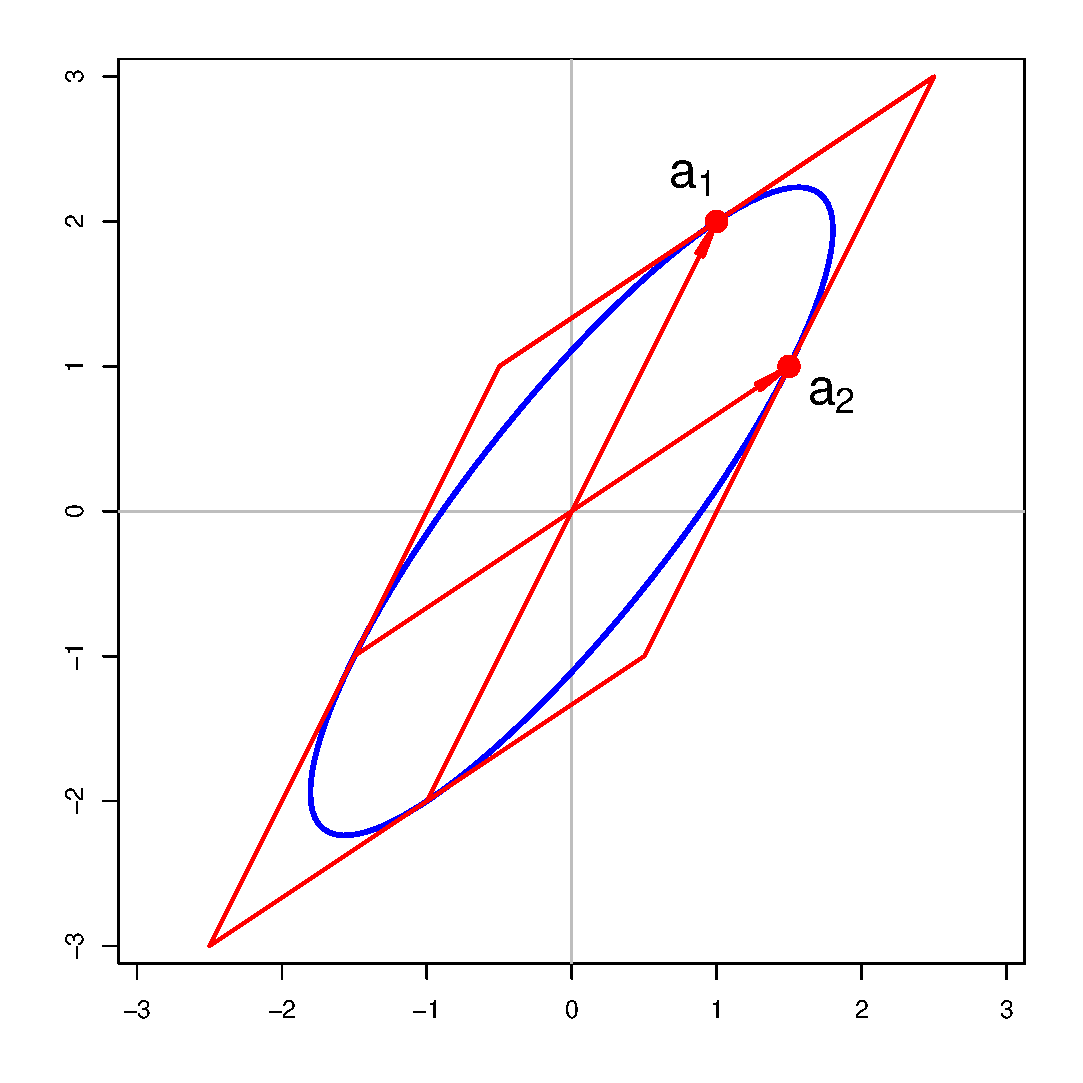
\includegraphics[width=1\linewidth]{fig/conjugate1}
 \end{minipage}%
 \hfill
 \begin{minipage}[b]{.49\linewidth}
  \centering
  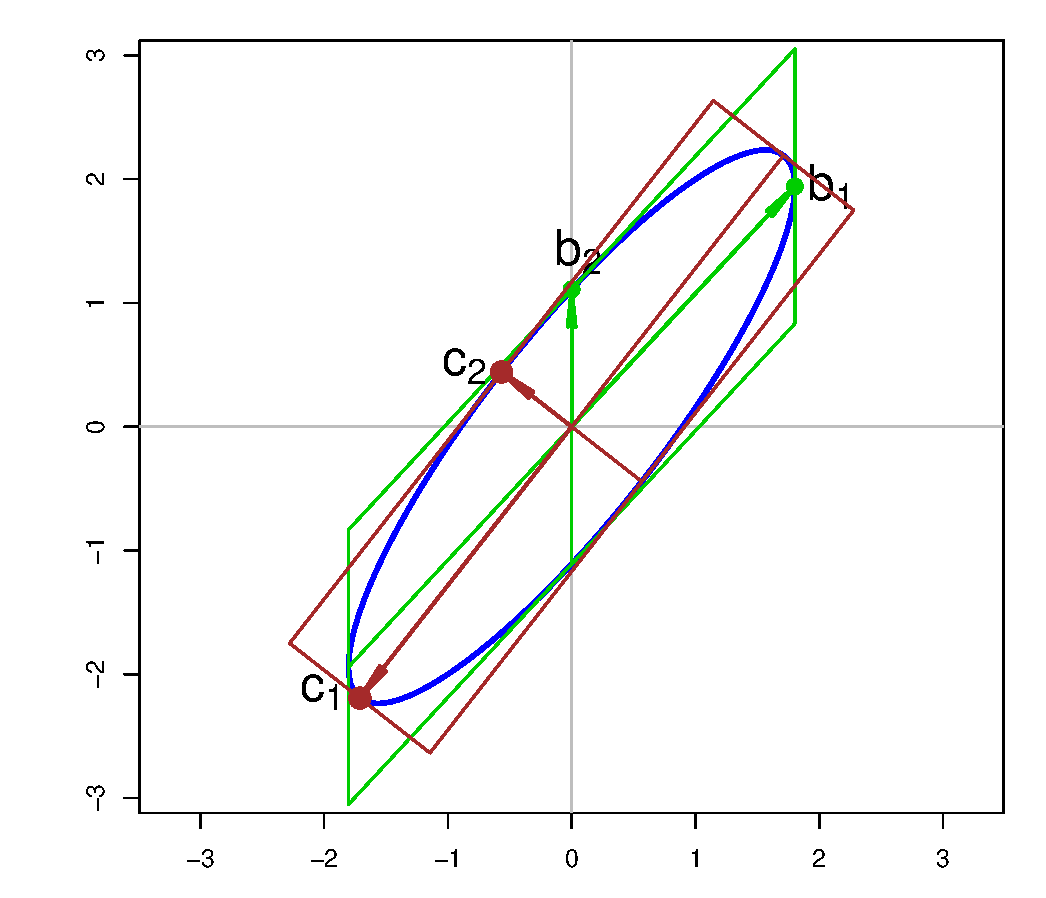
\includegraphics[width=1\linewidth]{fig/conjugate2}
 \end{minipage}
\caption{Conjugate axes of an ellipsoid with various factorizations of $\mat{W}$ and corresponding
basis vectors.
The conjugate vectors lie on the ellipsoid, and their tangents can be extended to form a parallelogram framing it.
Left: for an arbitrary factorization, given in \eqref{eq:fac1}.
Right: for the Choleski factorization (green, $b_1, b_2$) and the principal component factorization (brown, $c_1, c_2$).
}
\label{fig:conjugate}
\end{figure}
For
$p=2$
this result is illustrated in \figref{fig:conjugate} (left)
in which

\begin{equation}\label{eq:fac1}
\mat{A}=\left[ \begin{matrix}
   \vec{a}_{1} & \mat{a}_{2}  \\
\end{matrix} \right]=\left[
\begin{matrix}
   1 & 1.5  \\
   2 & 1  \\
\end{matrix} \right]
\mbox{   }\Rightarrow\mbox{   }
\mat{W}=\mat{A A\trans}=
\left[ \begin{matrix}
   3.25 & 3.5  \\
   3.5 & 5  \\
\end{matrix} \right]
\period
\end{equation}

Consider the inner-product space with inner product matrix 	
$\mat{W}^{-1}=\left[ \begin{matrix}	
1.25 & -0.875 \\	
-0.875 & 0.8125 \\	
\end{matrix} \right]
$ and inner product	
\begin{equation*}
\left\langle \vec{x},\vec{y} \right\rangle =\vec{{x}'W}^{-1}\vec{y} \period
\end{equation*} 	
Because	
$\mat{A}\trans \mat{W}^{-1}\mat{A}
=\mat{A}\trans\left( \mat{A}\mat{A}\trans \right)^{-1}\mat{A}
=\mat{A}\trans(\mat{A}\trans)^{-1}\mat{A}^{-1}\mat{A}
=\mat{I}
$,
we see that
$\vec{a}_{1}$
and	
$\vec{a}_{2}$	
are orthogonal unit vectors (in fact, an orthonormal basis) in this inner product:	

\begin{eqnarray*}
\left\langle \vec{a}_{i},\vec{a}_{i} \right\rangle & = & \vec{{a}\trans}_{i}\mat{W}^{-1}\vec{a}_{i}=1	 \\
%	
\left\langle \vec{a}_{1},\vec{a}_{2} \right\rangle & = &\vec{{a}'}_{1}\mat{W}^{-1}\vec{a}_{2}=0 \period
\end{eqnarray*}


Now, if $\mat{W}=\mat{B{B}\trans}$ is any other factorization of
$\mat{W}$,
then the columns of
$\mat{B}$
have the same properties as the columns of
$\mat{A}$.
Particular factorizations yield interesting and statistically useful sets of conjugate axes.
The illustration in \figref{fig:conjugate} (right) shows two such cases with special properties:
In the Choleski factorization (shown in green), where
$\mat{B}$ is lower triangular, the last conjugate axis, $\vec{b}_2$, is aligned with the coordinate
axis $\vec{x}_2$.  Each previous axis ($\vec{b}_1$, here) is the orthogonal complement to
all later axes in the  inner-product space of
$\mat{W}^{-1}$.  
The Choleski factorization is unique in this respect, subject to a
permutation of the rows and columns of \mat{W}. 
The subspace $\{ c_1 \vec{b}_1 + ... + c_{p-1} \vec{b}_{p-1}  , c_i \in \mathbb{R}\}$, is the plane of the regression of the last variable on the others, a fact that generalizes naturally to ellipsoids that are not necessarily centerered at the origin.  %% added fact /GM  

In the principal-component (PC) factorization (shown in brown) $\mat{W}=\mat{C} \mat{C}\trans$, where
$\mat{C}=\mat{\Gamma \Lambda }^{1/2}$
and hence
$\mat{W}=\mat{\Gamma \Lambda {\Gamma }'}$
is the spectral decomposition of
$\mat{W}$. Here, the ellipse axes are orthogonal in the space of the ellipse
(so the bounding tangent parallelogram is a rectangle) \emph{as well as} in the inner-product space of
$\mat{W}^{-1}$. The PC factorization is unique in this respect (up to reflections of the axis vectors).

As illustrated in \figref{fig:conjugate}, each pair of conjugate axes has a corresponding bounding tangent
parallelogram. It can be shown that all such parallelograms have the same area
and equal sums of squares of the lengths of their diameters.
